%\chapter{Belief Model}
\subsection{Belief Model}
\label{sec:uavBelief}
The belief model is the fundamental piece that allows the swarm to function as a cohesive group instead of many individuals in the same local area.  The belief model consists of data about all cells in the world grid and data about all known targets.  Each UAV has its own unique belief about the current state of the world.  Periodically the UAVs broadcast their belief to everyone nearby within communications range.  When a UAV receives another UAV's belief model the receiver merges the incoming data into their own internal belief model.  By this mechanism data is shared and propagated throughout the swarm.  Therefore the communication range of each UAV is a limiting factor in the effectiveness of the swarm.  Like all team based exercises effective communication is critical to success.  Figure~\ref{fig:comm_ranges} shows the communication ranges of the blue swarm as cyan circles around the swarm members.  In this figure only the two swarm members in the bottom left have overlapping communication ranges so only those two are sharing belief data at this moment in the simulation.

%\end{multicols*}

%\begin{multicols*}{2}

%\section{Cell Beliefs}
\subsubsection{Cell Beliefs}
Prior to beginning the mission the geographic area is tessellated into a rectangular grid of $M$ rows and $N$ columns.  The actual physical size of the cells is irrelevant to the algorithm.  However, scanning half a cell and declaring it empty while a target sits in the other half is erroneous.  Therefore a constraint exists such that the grid cells must be small enough so that the smallest field-of-view of all the sensors must be able to completely encompass a grid cell in a single sensor frame.  This constraint prevents the noted error condition.

\begin{figure}[H]
	\centering
	%\includegraphics[width=\linewidth,height=\textheight]{imagefile}
	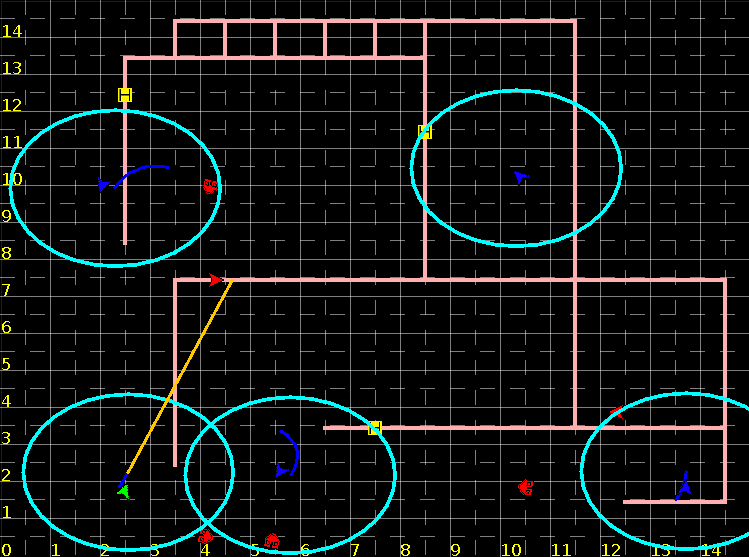
\includegraphics[scale=0.3]{comm_ranges.png}
	\caption{UAV communication ranges at $10\%$}
	\label{fig:comm_ranges}
\end{figure}

Each cell in the world grid is identified by a row and column index.  Each cell contains a probability of being empty, $P(empty)$, and a timestamp of when this data was last updated.  This is commonly called a Grid Based Occupancy Map. The probability value is updated in a Bayesian fashion by sensor scans during each time step of the simulation similar to~\parencite{waharte}.  
	
The Bayesian Inference update equation is shown in equations~\ref{eq:bayesianEmptyDenom} and \ref{eq:bayesianEmpty} where $P_{t}(T_{i})$ is the current probability at time $t$ that a target $T$ of the $ith$ target type is present and  $P_{t-1}(T_{i})$ is the previous timestep's probability that a target $T$ of the $ith$ target type is present.  These values are taken from the Target Belief models described in the next section.  If no Target Belief is located in the cell being updated then these probabilities are set to zero.  $P(S_{i}|T_{i})$ is the probability of a sensor $S$ detecting target type $i$ and correctly perceiving it as a type $i$.  

Note in equation~\ref{eq:bayesianEmptyDenom} that the reverse of $P(S_{i}|T_{i})$ is used by subtracting it from $1$.  This is because we need the probability that the sensor missed detecting the target given that the target was actually present.  

\begin{equation}
\label{eq:bayesianEmptyDenom}
%P(miss) = \prod_{j=0}^{\text{All Target Types}} (1 - P(S_{j}|T_{j})) * P_{t-1}(T_{j})
P(miss) = \sum_{i=0}^{\text{All Target Types}} (1 - P(S_{i}|T_{i})) * P_{t-1}(T_{i})
\end{equation}

\begin{equation}
\label{eq:bayesianEmpty}
P_{t}(empty) = \frac{P(S_{e}|T_{e})*P_{t-1}(empty)}{ P(S_{e}|T_{e})*P_{t-1}(empty) + P(miss)}
\end{equation}


Similar to \parencite{jin}, the $P(empty)$ probability is then used to derive a Discrete Shannon Uncertainty value as described in \parencite{shannon} (also known as Shannon Entropy).  A Shannon Uncertainty curve is zero when $P(empty)$ is 0\% or 100\% since in those edges cases we know for certain if the cell is empty or not.  Conversely a Shannon Uncertainty curve is at its peak when we know nothing for certain when $P(empty)$ is 50\%.  Nominally a Shannon Uncertainty curve varies from zero to one when $P(empty) = 0.5$. The equation can be see in~\ref{eq:shannon} and is plotted in figure~\ref{fig:shannon}.
	
\begin{equation}
\label{eq:shannon}
\begin{aligned}
U = &-P(empty) * \log_{2}(P(empty)) - \\&( 1-P(empty) * \log_{2}(1-P(empty)))
\end{aligned}
\end{equation}


\begin{figure}[H]
	\centering
	%\includegraphics[width=\linewidth,height=\textheight]{imagefile}
	\includegraphics[scale=0.4]{shannon.png}
	\caption{Shannon Uncertainty}
	\label{fig:shannon}
\end{figure}

%\end{multicols*}

%\begin{equation}
%\label{eq:shannon}
%U = -P(empty) * \log_{2}(P(empty)) - ( 1-P(empty) * \log_{2}(1-P(empty)))
%\end{equation}

%\begin{multicols*}{2}



The goal of the mission is to find all of the targets and destroy them.  In order to guarantee that all targets have been found the UAVs must reduce the Shannon Uncertainty of each world cell to 0 in their shared belief model.  In practice the world cells are never all driven to 0 at once.  There is a global certainty decay rate that is applied to the cell beliefs at every time step.  It slowly drives $P(empty)$ back to 50\% over time.  This models the fact that unless a UAV is watching a cell they cannot know with 100\% certainty what is going on within that cell.  There is a chance that a moving target that has somehow evaded detection could be occupying a previously scanned world cell location.  So instead of requiring the uncertainty of all world cells to be at 0\% to end the mission we only require that all cells be driven below a user defined threshold percentage.

%A more accurate dispersion of uncertainty would require all UAVs in the swarm to understand the kinematic limits of every target type in the mission area.  Upon detection and subsequent sensor loss of a mobile target, uncertainty should radiate outward from the target's last known location.  The rate and directionality of uncertainty propagation would be computed using the known maximum speed and turning characteristics of the target's suspected type. This more accurate technique was not utilized in this model for two reasons.  One reason is that this increase in accuracy comes with an increase in algorithm complexity and computing requirements.  The goal of this work is to obtain swarming behavior with minimal logic and this added complexity negates that goal.  The second reason is because of the target data requirements.  Collecting and formatting this information for all of the pre-existing legacy vehicles in the swarm would be an additional burden on software retrofitting tasks.  It also poses additional intelligence gathering requirements before every deployment of the swarm.  Therefore the naive global decay rate for uncertainty, while not fully accurate, is feasible and usable.



%\section{Target Beliefs}
\subsubsection{Target Beliefs}
When a UAV detects something that might be a target it adds a Target Belief to its Belief Model.  The Target Belief contains an estimation of the target's location and orientation.  It also contains a list of all possible target types and an associated probability that the detected target is the corresponding type of target. The list of target type probabilities within a Target Belief always sum up to one.  At initialization all target types are equally likely.  As time progresses and more sensor detection attempts of the target are completed the probabilities per target type will converge to a single type.  As with Cell Beliefs the probabilities for target type's are updated using a Bayesian Inference system.  

%is the Detected Target Type from a sensor scan and $TT$ is a Target Type. $P_{TT}(x)$ is the probability that the scanned target's type is the $x$ type.  This equation is applied for every suspected target type returned from a sensor scan.  After all of the sensor's possible target type results have been evaluated then the probabilities for all target types are normalized in the Target Belief.\textbf{TODO: mulitcol format}

%	P(\text{Detected Target Type} Y) = \frac{P(detect tgt type y) * P(prev belieft tgt Y exists)}{\sum_{T_{0}}^{Num Tgts}P(detect X as Y) * P(Prev beleif of X)}
%	P(\text{Target is detected type}) = \frac{P(\text{Detecting Target Type}) * P(\text{Previous Target is detected type})}{\sum_{i=T_{0}}^{All types}d}

%P(\text{(Mis)Classifying T_{i} as detected type}) * P(\text{Previous Target is T_{i}})

%\end{multicols*}

%\begin{equation}
%\label{eq:bayesian_verbal}
%P_{TT}^{'}(DTT) = \frac{ P(\text{Detecting }TT) * P_{TT}(DTT)} {\sum_{i=0}^{\text{Target types}}P(\text{ (Mis)Classifying } i \text{ as } DTT) * P_{TT}(i)}
%\end{equation}

\begin{equation}
\label{eq:bayesianTgt}
P_{t}(T_{i}) = \frac{P(S_{i}|T_{i})*P_{t-1}(T_{i})}{ \sum_{j=0}^{\text{All Target Types}}P(S_{j}|T_{i}) * P_{t-1}(T_{j}) }
\end{equation}

\begin{equation}
\label{eq:probsNormalize}
\left( \sum_{j=0}^{\text{All Target Types}}P_{t}(T_{j})\right)  = 1
\end{equation}

%	P_{TT}(DTT) = \frac{ P(\text{Detecting }TT) * P_{TT}(DTT)}  {ddd}

The Bayesian Inference update equation for Target Beliefs is shown in equation~\ref{eq:bayesianTgt}.  The parameters in equation~\ref{eq:bayesianTgt} are the same as for Cell Beliefs with the addition of $P(S_{j}|T_{i})$ which is the probability of mis-perceiving a detection of a target type $i$ as a target type $j$.  This equation is applied for every suspected target type returned from a sensor scan of a world cell. After all of the sensor's possible target type results have been evaluated then the probabilities for all target types are normalized in the Target Belief such that equation~\ref{eq:probsNormalize} holds true.  The values for $P(S_{x}|T_{x})$ used in this work are listed in Table~\ref{tab:snsrTgtProb}.



The Target Belief's orientation is updated upon each sensor scan with a simple weighted average of the perceived heading and the previous estimated heading value.  The simulation generates the perceived heading values in sensor detections by applying a random noise error value on top of truth data.  The simulation assumes that all sensors can estimate a target's heading within $\pm45^{\circ}$ of truth as a baseline performance.  This error range is scaled by $H_{ij}$ (described back in section~\ref{sec:sensor_var_descriptions}) to model sensor accuracy. The error range is computed with equation~\ref{eq:hdg_err_rng}.  Equation~\ref{eq:rand_hdg_err} then randomly selects a positive or negative value ($Hdg_{err}$) in the error range.  The results of equation~\ref{eq:rand_hdg_err} is then added to the true heading ($Hdg_{t}$) of the target to create the perceived heading ($Hdg_{p}$) in simulated sensor detections.

\begin{equation}
\label{eq:hdg_err_rng}
Err_{rng} = 90^{\circ} * (1 - H_{ij})
\end{equation}

\begin{equation}
\label{eq:rand_hdg_err}
Hdg_{err} = (random() * Err_{rng}) - \frac{Err_{rng}}{2}
\end{equation}

\begin{equation}
Hdg_{p} = Hdg_{t} + Hdg_{err}
\end{equation}

%\begin{multicols*}{2}
In addition to estimated physical data about the target, Target Beliefs encapsulate information about the tasks performed on the target.  This tasking data is collectively called the Target Task Status.  This data is used for coordinating activities within the swarm.  Since the swarm of UAVs has no centralized control system to allocate task assignments this process must be done by mutual consent within the swarm.  Mutual consent is facilitated by means of a scoring system and enumeration control flags contained in a Target Task Status.  Each Target Belief contains a Target Task Status.  The Target Task Status denotes who is performing tasks on a target and if the task is still eligible for others to take over. The Target Task Status includes the following attributes.

\begin{description}
	\item [Monitor UAV ID] The ID of the UAV who has the best monitor score.
	\item [Monitor UAV Score] The best known score for monitoring the target.
	\item [Monitor Task State] An enumeration describing the current phase of task coordination for monitoring.
	\item [Monitor Update Timestamp] The time when the monitor data was last updated.
	\item [Attack UAV ID] The ID of the UAV who has the best attack score.
	\item [Attack UAV Score] The best known score for attacking the target.
	\item [Attack Task State] An enumeration describing the current phase of task coordination for the attack.
	\item [Attack Update Timestamp] The time when the attack data was last updated.
	\item [Target Destroyed Flag] A flag indicating if the target has been destroyed or not.
\end{description}

The Monitor Task State and Attack Task State enumerations control when and who may bid on tasks.  There are subtle differences in their uses between the monitor tasks and the attack tasks.  These are explained in detail in  section~\ref{sec:uncoordTaskingMyWork}.

\begin{description}
	\item [NO TASK] This is the initial null condition given to the monitor and attack tasks.  In the monitor case it means the target was just discovered and no one has had a chance to process it.  In the attack case it means no one has confirmed that the target should be destroyed.
	\item [Open] The task is open to any and all bids.  No one has attempted to claim the task yet.
	\item [Enroute] This means the UAV with the corresponding ID is on its way to the target to perform the corresponding task.  Anyone else could overrule if they have better score than current best UAV.
	\item [Performing] The UAV with the corresponding ID is now performing the action.  No one else may overrule or otherwise subsume the action without a special exemption.%regardless of their score.
	\item [Complete] The task has been completed by the UAV with the corresponding ID.  In the monitor case the target has been confirmed as destroyed.  In the attack case a weapon has been deployed but the target is not necessarily destroyed.
\end{description}

%\section{Merging Beliefs}
\subsection{Merging Beliefs}
\label{sec:mergingBeliefs}
Each UAV in the swarm periodically broadcasts its internal Belief Model.  The model is shown in Object Diagram format in figure~\ref{fig:belief_object}.  The entire model is encoded and transmitted to all other swarm members within communications range.   When a UAV receives another swarm member's belief model it must be merged with the receiver's internal belief.  No UAV completely trusts any other UAV in the swarm.  All data is merged in a weighted or filtered fashion.  No data is copied 100\% as-is since there are no guarantees that any one UAV is perfectly correct about anything.  The merging process in this work is an implementation of the Fusion Update technique described in~\parencite{shem} for merging multiple values of uncertainty.
	
%\textbf{TODO: Multicol formatting issue}
%The entirety of the Belief Model is shown in figure~\ref{fig:belief_object} in an Object Diagram.

	
%\textbf{TODO: Future work: Sensor type expertise should weigh into this}.

Merging Cell Beliefs is a simple process and is described in algorithm~\ref{alg:mergeCell} in section~\ref{sec:algorithms}.   In short the receiving UAV compares every single world cell with its counterpart in the sending UAV's data.  If the last update timestamp of the incoming cell data is more recent than the currently stored data then the cell data is merged.  The merge process is a weighted average.  When the merge occurs the receiving UAV's timestamp is set to the timestamp of sending UAV's data.  This prevents future belief broadcasts from the same sending UAV to trigger another re-merging of the exact same cell data.  This also prevents the same data from re-merging if a third party UAV forwards the belief data. 

%Other alternative algorithms exist for for merging the belief data.  A Bayesian system is intractable because it would require every UAV in the swarm to know all of the characteristics of every other sensor in the swarm.  Every sensor detection would have to be encode in the belief data including all of the relative geometries between the sensor and target.  This would let the receivers recompute the entire world model with complete information.  The data transmission requirements and processing requirements for this merging system are enormous.  These requirements defeat the purpose of retrofitting legacy hardware platforms into a swarm but it would provide perfect synchronization between belief models.

A pure Bayesian approach for merging cell beliefs is intractable because it would require every UAV in the swarm to recompute the word model from the entire history of all sensor readings every time new information was received.  This would defeat the goal of a simple algorithm that could easily retrofit legacy hardware platforms into a swarm.


%Another alternative is to choose the belief data with the lower uncertainty.  The UAV with a lower uncertainty should have newer information, more sensor readings, or readings from better sensor(s).  If all of the sensors in the swarm had similar performance characteristics this would be a suitable method.  Problems arise when very poor sensors and very high quality sensors work together in the swarm.  No information about which sensor type performed a detection to update the belief model is encoded.  The belief model on the poor quality UAV may think it has very low certainty but in actuality it's just a collection of poor readings that are heavily mistaken.  The belief from a poor quality sensor might say that the $P(empty)$ of a cell is 10\% while the belief from a high quality sensor might say that the $P(empty)$ of that same cell is 90\%.  Both $P(empty)$ yield an uncertainty of roughly 0.4.  So which of these is the better one to choose in this case?  Without a better model of uncertainty that can account for these quality discrepancies this is not a viable alternative.

%From sauter arguing against the above paragraph:
%A fuller explanation of my comments in the doc regarding your argument against using the maximum certainty cell for the merged beliefs is included here. I still believe your explanation is wrong. Let's look at a specific example. Say I have a lousy sensor (only a little better than a random sensor) and two target types (T0 and T1). The sensor identifies the targets with the following true and false positive rates:
%P(S1|T1) = 0.61
%P(S0|T1) = 0.39
%P(S0|T0) = 0.61
%P(S1|T0) = 0.39

%I also have a sensor that is much better than random It has the following true and false positive rates:
%P(S1|T1) = 0.8
%P(S0|T1) = 0.2
%P(S0|T0) = 0.8
%P(S1|T0) = 0.2

%I get three bad readings from the first sensor on a target of type T1 (i.e. the sensor reads S0, S0, S0). The probability of getting three bad sensor readings like that is 0.39^3 or only 5.9%. If I run the Bayes model on those three sensor readings it will say that the probability that the target is of type T0 is 79%. 

%Now I take 1 sensor reading with the good sensor. It also gives the wrong reading saying its a T0 type. The probability that it will give that wrong reading is actually 20%. The Bayes model says that the probability of it being a target of type T0 is 80% (same as the bad sensor). 

%Which do I believe? You say the better sensor, but the better sensor actually had a much higher probability of resulting in the very wrong estimate that P(T0)=80% while the lousy sensor had only a 5.9% chance of reaching that same wrong estimate! As you can see, the real differentiator is the number of readings involved, not the quality of the sensor.
%End from Sauter

Using a weighted average is not a perfect solution but it is simple, intuitive, and easy to derive when comparing sensor and target type pairings.  It also prevents each UAV from having to know the details about every other UAV or sensor in the swarm.  The only one who knows all of the capabilities of the swarm is the human operator. It puts the responsibility on the swarm operator to give a relative strength per sensor and target type pairing.  It lets the operator set whether the UAV is extremely trusting of external data about a target or distrustful of external data about a target.

\end{multicols*}
\begin{figure}[H]
	\centering
	%\includegraphics[width=\linewidth,height=\textheight]{imagefile}
	\includegraphics[scale=0.75]{belief_object.png}
	\caption{Belief Model Object Diagram}
	\label{fig:belief_object}
\end{figure}
\begin{multicols*}{2}


Table~\ref{tab:exampleCellMerge} shows an example of merging a single cell.  At some time in the simulation UAV 1 believes cell $[2, 6]$ has a 20\% of being empty (or in other words an 80\% chance that something is there). This probability was last updated at time 1234.  UAV 1 has broadcasted this belief data and UAV 2 has received it.  UAV 2 believes there is a 50\% chance that the same cell is empty but this data was last updated a long time ago at time 22.  Therefore UAV 2 will merge UAV 1's data for this cell.  Since alpha is set to 0.6 the new $P_{2,6}(empty)$ for UAV 2 is $0.6*(0.2) + (1-0.6)*(0.5)=0.32$.  After the merging is complete UAV 2's $P(empty)$ value is set to $0.32$ and the last update timestamp is set to UAV 1's timestamp.

\begin{table}[H]
	\caption{Example cell merging with $alpha=0.6$}
	\centering
	\rowcolors{1}{lightgray}{white}
	\label{tab:exampleCellMerge}
	\begin{tabular}{|r|c|c||c|c|}
		\hline
		& \multicolumn{2}{c||}{Before Merge} & \multicolumn{2}{c|}{After Merge} \\
		\hline
		UAV             & 1   & 2                            & 1   & 2 \\
		\hline
		$P_{2,6}(empty)$& 0.2 & 0.5                          & 0.2 & 0.32 \\
		\hline
		Timestamp       & 1234& 22                           & 1234& 1234 \\
		\hline
	\end{tabular}
\end{table}

Merging Target Beliefs is more complicated but uses a similar weighted averaging technique as merging Cell Beliefs.  The model in this paper assumes that the UAVs are able to perform target track fusion (also known has cross-track correlation) amongst themselves and assign each track a unique ID such as in~\parencite{stroupe}, \parencite{barooah}, and~\parencite{spillings}.  This process is outside the scope of this paper.
			
As stated earlier Target Beliefs have an estimated location, orientation, and list of target type probabilities.  Now we assume they also have a unique identifier assigned by the target track fusion process.  This unique identifier is used as a first pass comparison filter when merging Target Belief data.  If the receiving UAV does not have any data for the incoming Target Belief it simply copies it verbatim.  If the receiving UAV already has data for the Target Belief then a more detailed inspection is required.  Target Beliefs only get merged if the received data is newer than the currently stored data.  In this case the estimated target orientation, position, and list of type probabilities are all averaged with a user defined weighting against the incoming data.  The formal algorithm is defined in algorithm~\ref{alg:mergeTarget}.

The Target Task Status within a Target Belief is also merged with incoming data.  Instead of performing weighted averages logic must be applied to determine if the task status data is still live and active or if the data is transmitted for historical reference only.  The formal algorithm is defined in algorithm~\ref{alg:mergeTaskStatus} of section~\ref{sec:algorithms}.